% Define the module top matter
% This gets used to create the chapter title page
% NOTES:
%  * When multiple people have authored or contributed to the module, simply use a LaTeX line break
%    (a double-backslash: \\) at the end of each person.
%  * If you don't want this information shown on the module chapter page, simply remove the lines
%    within the \setModuleAuthors{} and \setModuleContributions{} environments
\setModuleTitle{Introduction to Snakemake}
\setModuleAuthors{%
  Nathan S. Watson-Haigh \mailto{nathan.watson-haigh@adelaide.edu.au}
}
%\setModuleContributions{%
%  John Doe \mailto{john.dow@example.com}%
%}

% BEGIN: Module Title Page
% This simply uses the above information and creates a module chapter page
% NOTES:
%  * The chapter page will always appear on odd numbered page
\chapter{\moduleTitle}
\newpage
% END: Module Title Page


% BEGIN: KLOs
% Key Learning Outcomes (KLOs) are an important aspect of any learning/training. They provide
% valuable infomation about what the trainee will have learned, what they will be able to do or know
% abouti at the end of the module. Unlike objectives which are more trainer oriented, KOLs are
% focused on the learner.
% At the end of the module, the KLOs can be used to develop criteria for writing an assessment to
% see if the trainees knowledge/skills have improved as a result of the module.
% 
% Search online for information on how to write KLOs. e.g.
% http://www.teaching-learning.utas.edu.au/__data/assets/word_doc/0014/23333/Learning-outcomes-v9.1.doc
\section{Key Learning Outcomes}

After completing this module the trainee should be able to:
\begin{itemize}
  \item Install Snakemake in a conda environment
  \item Execute a Snakemake workflow
  \item Use the provided ``profile'' to execute jobs on a compute cluster
  \item Write simple Snakemake rules capable of generating some output(s) by executing some code which perates on some input(s)
\end{itemize}
% END KLOs

% BEGIN: Resources Used
% This section can be used to describe the tools and data used during the module. It helps to act as
% a future reference to the trainee
\section{Resources Required}

For the purpose of this training you need access to:

\begin{itemize}
  \item A compute cluster with the \texttt{module} command available to you for loading software
  \item Singularity (\url{https://sylabs.io/singularity/}) - available as a module on the above cluster
  \item Conda(\url{https://www.anaconda.com/distribution/}) - available as a module on the above cluster
\end{itemize}


\subsection{Tools Used}
\begin{description}[style=multiline,labelindent=0cm,align=left,leftmargin=0.5cm]
  \item[Snakemake]\hfill\\
    \url{https://snakemake.readthedocs.io}
  \item[Graphviz]\hfill\\
    \url{https://www.graphviz.org}
\end{description}

\section{Useful Links}
 
\begin{description}[style=multiline,labelindent=0cm,align=left,leftmargin=0.5cm]
  \item[Slurm Documentation]\hfill\\
    \url{https://slurm.schedmd.com/documentation.html}
\end{description}

\newpage
% END: Resources Used

%========================
\section{Snakemake is Like Making Sunday Dinner}
%========================

The way Snakemake approaches running workflows is a bit like the way you prepare for dinner/tea. First, you think about what you
want for dinner/tea, say a Sunday roast. To create the Sunday roast, you need meat and vegetables, all of which need preparing
(e.g. peeling and seasoning). If you haven't got an ingredient, you go out to the shop and buy it.

With Snakemake, you decide what output files you want to create, say some BAM files. To create the BAM files, you need FASTQ files
and a reference genome, all of which need preparing (e.g. quality/adapter trimming and indexing). If you haven't got those files,
you need to create them.

% TODO: Create DAG of Sunday Dinner

%========================
\section{Setting Up Your Environment}
%========================

For the purpose of the workshop we will be working on the head node of an HPC cluster running slurm (\url{https://slurm.schedmd.com/documentation.html}).
This is the most likely infrastructure that fellow bioinformaticians already find themselves using
on a regular basis. We also assume that the cluster provides the \texttt{module} command for you to
load software and the modules \texttt{Anaconda3} and \texttt{Singularity} are available to use.

The execution of the Snakemake workflow will actually take place on the cluster head node with jobs
being submitted to Slurm for queing and processing. From the head node, Snakemake will monitor the
submitted jobs for their completion status and submit new jobs as dependent jobs complete sucessfully.

%------------------------
\subsection{Installing Snakemake}
%------------------------

The recommended installation route for Snakemake is through a conda environemnt
(\url{https://snakemake.readthedocs.io/en/stable/getting_started/installation.html}). As such, you need
Anaconda3, usually avaiable to you on your cluster via the module system.

\begin{steps}
\begin{lstlisting}
# We use a specific version for reproducibility reasons
# Find the latest version: https://anaconda.org/search?q=snakemake
SNAKEMAKE_VERSION="5.5.4"

# Load miniconda
module load \
  miniconda3-4.6.14-gcc-5.4.0-kkzv7zk

#####
# One-time commands
#####
# Integrate conda into bash
conda init bash
. ${HOME}/.bashrc

# Change the default location into which conda saves packages
# and environments
conda config --prepend pkgs_dirs /shared/${USER}/.conda/pkgs
conda config --prepend envs_dirs /shared/${USER}/.conda/envs

# Change the default channels used for finding software and
# resolving dependencies
conda config --add channels defaults
conda config --add channels bioconda
conda config --add channels conda-forge
#####
\end{lstlisting}

\end{steps}

\begin{warning}

Do NOT run the following command! This is provided for future reference so you know how to Install Snakemake on another system. Rather than
creating the conda environment from scratch, we'll simply copy a pre-existing directory so we save time, and possible headaches.

\begin{lstlisting}
# Install snakemake using conda
# This might take 5-10mins
conda create \
  --name snakemake \
  --yes \
  snakemake=${SNAKEMAKE_VERSION:-5.5.4}
\end{lstlisting}

Snakemake installation is now complete.

\end{warning}

\begin{steps}

For the purposes of this workshop, simply copy the following \texttt{.conda} directory and you
will have Snakemake setup and ready to go:

\begin{lstlisting}
mkdir --parents /shared/${USER}
cp --recursive \
  /shared/ubuntu/.conda \
  /shared/${USER}/
\end{lstlisting}

All that is left to do is to activate the environment which will make \texttt{snakemake} available on the command line:

\begin{lstlisting}
# Activate the conda environment
conda activate snakemake
\end{lstlisting}

Integrate Snakemake autocompletion into bash:

\begin{lstlisting}
complete -o bashdefault -C snakemake-bash-completion snakemake
\end{lstlisting}

Test if Snakemake is actually working:

\begin{lstlisting}
snakemake --version
\end{lstlisting}

\end{steps}

If you experience problems with the installation, head to the \hyperref[sec:snake_trouble]{Troubleshooting} section for help.

\begin{bonus}

While waiting for others to catch up, why not have a look into how you would go about updating \texttt{Snakemake}
within this conda environment if there is a new version available.

\begin{answer}
\begin{lstlisting}
conda update \
  snakemake
\end{lstlisting}
\end{answer}

\end{bonus}


%========================
\section{Your First Snakemake Workflow}
%========================

To get started with Snakemake, all you need to do is create a \texttt{Snakefile} (note the capitalisation) containing a rule
which specifies how to create an output file.

Setup a working directory for this task:

\begin{lstlisting}
mkdir --parents /shared/${USER}/snakemake/hello
cd /shared/${USER}/snakemake/hello
\end{lstlisting}

Create a file called \texttt{Snakefile} and add the following content:

\begin{lstlisting}
rule hello_world:
  output:
    "Hello/World.txt",
  shell:
    """
    echo "Hello, World!" > {output}
    """
\end{lstlisting}

You can now run this workflow in one of 3 ways:

\begin{lstlisting}
# Request Snakemake to generate the specific output file
# "Hello/World.txt"
snakemake Hello/World.txt

# Request Snakemake to execute the specific rule "hello_world"
snakemake hello_world

# Request Snakemake to execute the first rule in the Snakefile
snakemake
\end{lstlisting}

\begin{questions}

What happens if you run one of the above commands two or more times? Why?

\begin{answer}
Snakemake found the requested output file was already there so decided not to regenerate it.
\end{answer}

\end{questions}


%========================
\section{Generalising Rules with Wildcards}
%========================

The original \texttt{hello\_world} rule wasn't very flexible. We couldn't say ``Hello, World!'' in Spanish, Polish
or French. However, we can generalise the rule using ``wildcards'' (\url{https://snakemake.readthedocs.io/en/stable/snakefiles/rules.html#wildcards}):

\begin{lstlisting}
rule hello_world:
	output:
		"{cheer}/{world}.txt",
	shell:
		"""
		echo "{wildcards.cheer}, {wildcards.world}!" > {output}
		"""
\end{lstlisting}

Now we can use whatever language we want:

\begin{lstlisting}
# In English - nothing should be done since the file
# already exists
snakemake Hello/World.txt

# In Polish
snakemake Czesc/Swiat.txt

# In French and Spanish at the same time
snakemake Monde/Monde.txt Ciao/Mondo.txt
\end{lstlisting}

Take a look at the files created and their contents:

\begin{lstlisting}
tree ./
cat */*.txt
\end{lstlisting}

%========================
\section{Submitting Jobs to Slurm}
%========================

By default, Snakemake executes jobs on the same computer on which it is running. For Snakemake to be able to
submit jobs to a cluster resource management/queuing system, such as Slurm, we can use a ``profile'' which
convieniently contains scripts for job submission and monitoring as well as setting some additional Snakemake
command line arguments so it can ``talk'' to a cluster backend.

To avoid having to delve into implementing our own ``profile'' for use with our Slurm cluster, we have created
a Slurm profile ready for you to use. So lets grab it:

\begin{lstlisting}
# Ensure a working directory exists and move into it
mkdir --parents /shared/${USER}/snakemake/tutorial
cd /shared/${USER}/snakemake/tutorial

# Clone the Snakemake template repository from GitHub
git clone https://github.com/UofABioinformaticsHub/snakemake_template ./

# Checkout the "hello" branch
git checkout hello
\end{lstlisting}

The \texttt{Snakefile} in this branch of the repository is the same ``Hello, World!'' example you created above,
with wildcards. Lets see how we use the provided ``profile'' to get Snakemake to submit jobs to Slurm:

\begin{lstlisting}
snakemake \
  --profile profiles/slurm \
  Hello/World.txt Czesc/Swiat.txt Monde/Monde.txt Ciao/Mondo.txt

# See what files we have
tree
\end{lstlisting}

If the \texttt{STDOUT} and \texttt{STDERR} of the command(s) in a rule are not explicitly sent to a file, then they will
end up in Slurm's log file for a particular job which is normally something like \texttt{slurm-<job\_id>.out}. This isn't
that helpful for debugging purposes, so the provided profile changes this to \texttt{logs/<rule\_name>/<wildcards>.out}
e.g. \texttt{logs/hello\_world/cheer=Ciao,world=Mondo.out}. See:

\begin{lstlisting}
tree logs/
\end{lstlisting}

We've finished with this simple ``Hello, World!'' example, so cleanup after yourself:

\begin{lstlisting}
snakemake \
  --delete-all-output \
  Hello/World.txt Czesc/Swiat.txt Monde/Monde.txt Ciao/Mondo.txt

# See what files we have
tree
\end{lstlisting}

%========================
\section{Reimplementing a Workflow in Snakemake}
%========================

A bioinformatic ``pipeline'' is commonly a single, monolithic bash script which performs all the tasks which need
to be performed. For example, someone might have written a script for performing the following tasks:

\begin{itemize}
  \item Run FastQC across all the raw read files
  \item Adapter, quality, and read length filtering using Trimmomatic
  \item Aggregating FastQC reports from the raw reads using MultiQC
  \item Index the reference FASTA file
  \item Perform a \texttt{bwa-mem} read alignment
\end{itemize}

We will walk you through the steps of reimplementing the first few steps of the above script into a Snakemake workflow. Along the way,
we will introduce the core concepts of Snakemake and then ask you to reimplement the \texttt{bwa-mem} step yourselves. For those
working quickly, you will have the opportunity to reimplement the \texttt{multiqc} step. This will provide you with a foundation
for you to be able to convert your own workflows into Snakemake rules and begin reaping the rewards of being able to run your analyses
in Snakemake.

%------------------------
\subsection{Getting the Code}
%------------------------

We have the monolithic script available for you on the \texttt{walkthrough} branch, switch to it and have a look:

\begin{lstlisting}
git checkout walkthrough

less analysis.sh
\end{lstlisting}

While the author of such a script should be commended for their efforts in documenting their analysis using a script,
it has several significant limitations:

\begin{description}[style=multiline,labelindent=0cm,align=left,leftmargin=0.5cm]
  \item[Not parallelised]\hfill\\
    Loops over input files, executing independant commands in sequential order
  \item[Resources over-specified]\hfill\\
    The compute resources needed by the script are dictated by the command(s) with the largest requirement(s)
  \item[Not idempotent]\hfill\\
    Significant programming logic is needed to wrap around commands to detect failures and only execute parts of the analysis which failed in earlier attempts
\end{description}

\begin{questions}

How might you modify the above script to:

\begin{itemize}
  \item Add new samples
  \item Rerun the script if you find one of the files generated is corrupt
  \item Include readgroup information at the \texttt{bwa-mem} step (\texttt{-b} argumanet)
\end{itemize}

How would you avoid rerunning commands which take a long time and already completed sucessfully
on a previous run e.g. the reference index, \texttt{bwa-mem} etc?

\begin{answer}

With difficulty!
Enter - workflow management systems like Snakemake or Nextflow.

\end{answer}

\end{questions}

%------------------------
\subsection{Getting the Data}
%------------------------

We've provided you with some real data whole genome sequencing (WGS) data from wheat together with a small chunk of the wheat genome.
The data set is small enough so each step in the analysis will take less than a couple of minutes to run. We have a copy of this data
available locally to save on badnwidth, time and the possibility we are detected as a DDoS attack on some poor remote server!

\begin{lstlisting}
# Get a copy of the data
cp --recursive \
  /shared/data/{raw_reads,references,misc} \
  ./

# Have a look at what files we'd provided
tree raw_reads references misc
\end{lstlisting}

%------------------------
\subsection{Implementation of BWA Indexing}
%------------------------

We have provided an out-of-the-box \texttt{Snakefile} capable of indexing the provided reference sequence, together with comments. Lets
have a bit of a play before we get around to actually running the workflow.

\begin{lstlisting}
less Snakefile

# These commands have the same effect
snakemake --dryrun all
snakemake --dryrun
\end{lstlisting}


\begin{questions}

Why doesn't this work:

\begin{lstlisting}
snakemake --dryrun bwa_index
\end{lstlisting}

\begin{answer}

Because the rule makes use of wildcards. Effectively, the wildcards are \texttt{NULL} values when
we specify the rule to run. We need to specify the target filenames and they will get matched against
the wildcards present in the defined \texttt{output}.

\end{answer}

Do we have to specify all 5 of the BWA index files in the \texttt{all} pseudo-rule?

\begin{answer}

No. Snakemake determines which rule needs to be run in order to create each of the 5 index files specified. Since all these files
are created by the \texttt{bwa\_index} rule, snakemake knows it only needs to run that rule once in order to create all 5 files.
We could easily have specified only one of the index files and this would have resulted in the same jobs being run.

\end{answer}

Why do we have to specify all 5 index files as \texttt{output} of the \texttt{bwa\_index} rule?

\begin{answer}

Because we want Snakemake to keep track of which files get generated as part of the workflow. This is how we are able to define
dependencies between rules.

\end{answer}

\end{questions}


The effect \texttt{--dryrun} is to simply show you what ``would'' be run, without actually running it. It's useful to ensure you're going to get
what you though, especially as your worflows get larger and more interconnected.

Another useful feature is to generate a directed acyclic graph (DAG) of the jobs which comprise the workflow and how they are linked together. Although
for this workflow is not yet that impressive, but we'll have a look at how we generate the DAG:

\begin{lstlisting}
snakemake \
  --dag \
| dot -Tpdf \
> dag1.pdf
\end{lstlisting}

\begin{figure}[H]
\centering
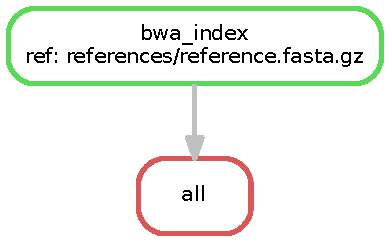
\includegraphics[width=0.8\textwidth]{handout/dag1.pdf}
\caption{DAG of jobs showing \texttt{bwa\_index} job dependant on the \texttt{all} pseudo-rule.}
\label{fig:dag1}
\end{figure}

%------------------------
\newpage
\subsection{Implementing FastQC}
%------------------------

Lets add a rule for performing FastQC on our input files. Looking at the \texttt{analysis.sh} file we see the following command
is executed for each \texttt{SAMPLE} while interating over the \texttt{SAMPLES} list:

\begin{lstlisting}
fastqc --threads 1 \
  raw_reads/${SAMPLE}_R1.fastq.gz \
  raw_reads/${SAMPLE}_R2.fastq.gz
\end{lstlisting}

This command can be converted into a Snakemake \texttt{rule} by adding the following rule to the \texttt{Snakefile}:

\begin{lstlisting}
rule fastqc:
	input:
		r1 = "raw_reads/{SAMPLE}_R1.fastq.gz",
		r2 = "raw_reads/{SAMPLE}_R2.fastq.gz",
	output:
		zip  = [
			"raw_reads/{SAMPLE}_R1_fastqc.zip",
			"raw_reads/{SAMPLE}_R2_fastqc.zip",
		],
		html = [
			"raw_reads/{SAMPLE}_R1_fastqc.html",
			"raw_reads/{SAMPLE}_R2_fastqc.html",
		],
	shell:
		"""
		fastqc --threads 1 {input.r1} {input.r2}
		"""
\end{lstlisting}

%........................
\subsubsection{Improving FastQC Parallelisation}
%........................

There are a few improvements we can make to the \texttt{fastqc} rule:

\begin{itemize}
  \item We don't need to process both the R1 and R2 read files with the same FastQC job. We can operate on one read file at a time.
        By doing this, Snakemake will be able to execute the FastQC job for each file in parallel.
  \item We want a convienient way of generating FastQC outputs for ALL samples without typing them all at the command line.
\end{itemize}

Change the \texttt{fastqc} rule to the following:

\begin{lstlisting}
rule fastqc:
	input:
		"raw_reads/{prefix}.fastq.gz",
	output:
		zip  = "raw_reads/{prefix}_fastqc.zip",
		html = "raw_reads/{prefix}_fastqc.html",
	shell:
		"""
		fastqc --threads {threads} {input}
		"""
\end{lstlisting}

Now run the same Snakemake dryrun command as before:

\begin{lstlisting}
snakemake --dryrun raw_reads/ACBarrie_R1_fastqc.html raw_reads/ACBarrie_R2_fastqc.html
\end{lstlisting}

%........................
\subsubsection{Rule-Specific Resource Specification}
%........................

The profile provided in this repository specifies default values for Slurm resources. However, it is possible to provide
rule-specific overrides so that jobs can make use of more time, memory, cores etc. The `cluster-configs/default.yaml` file is where
these settings can be modified.

\begin{lstlisting}
less cluster-configs/default.yaml
\end{lstlisting}

%........................
\subsubsection{Pseudo-Rules}
%........................

We can use ``pseudo-rules'' to define a list of target filenames for creation when we use the rule name as a ``target''. Pseudo-rules consist of just an \texttt{input} directive:

\begin{lstlisting}
rule all:
	input:
		"raw_reads/ACBarrie_R1_fastqc.html",
		"raw_reads/ACBarrie_R2_fastqc.html",
\end{lstlisting}

By convention, the first pseudo-rule in the \texttt{Snakefile} is called \texttt{all} and specifies all the output filenames of the workflow. This now
means we can execute a workflow in any of the following ways:

\begin{lstlisting}
# Not specifying a target will result in Snakemake executing the
# first rule in the Snakefile ("all" in this case)
snakemake --dryrun

# Explicityly request the "all" rule
snakemake --dryrun all
\end{lstlisting}

When workflows get larger and the lists of filenames get bigger, specifying long lists of filenames in pseudo-rules can start to feel cumbersome.
Since Snakemake syntax is an extension of Python, we can start to use some Python data structures and functions to help.

Add the following Python list of sample names (with most commented out for now) at the top of the file:

\begin{lstlisting}
SAMPLES = [
  "ACBarrie",
  "Alsen",
#  "Baxter",
#  "Chara",
#  "Drysdale",
#  "Excalibur",
#  "Gladius",
#  "H45",
#  "Kukri",
#  "Pastor",
#  "RAC875",
#  "Volcanii",
#  "Westonia",
#  "Wyalkatchem",
#  "Xiaoyan",
#  "Yitpi",
]
\end{lstlisting}

Add FastQC output files for all samples in the \texttt{SAMPLES} list, as well as both read files, as new targets to the existing \texttt{all} rule. We'll make use of the \texttt{expand()}
function to simplify things somewhat. The resulting \texttt{all} pseudo-rule should look like this:

\begin{lstlisting}
rule all:
	input:
		expand("references/reference.fasta.gz.{ext}",
			ext=['amb', 'ann', 'bwt', 'pac', 'sa']
		),
		expand("raw_reads/{SAMPLE}_{read}_fastqc.html",
			SAMPLE=SAMPLES,
			read=['R1', 'R2']
		),
\end{lstlisting}

Lets take a look at what jobs would be run if we run the whole workflow. Remember, the following commands are equivilent:

\begin{lstlisting}
# Explicitly run the "all" pseudo-rule
snakemake --dryrun all

# Run the first rule in the Snakefile. This should be the
# "all" rule by convention
snakemake --dryrun
\end{lstlisting}

Lets look at the DAG for the workflow:

\begin{lstlisting}
snakemake \
  --dag \
| dot -Tpdf \
> dag2.pdf
\end{lstlisting}

\begin{figure}[H]
\centering
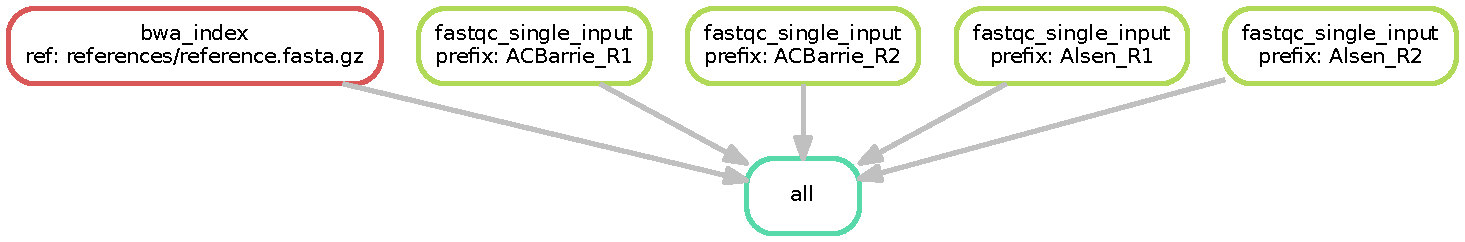
\includegraphics[width=0.8\textwidth]{handout/dag2.pdf}
\caption{DAG of jobs showing \texttt{bwa\_index} and several \texttt{fastqc} job dependant on the \texttt{all} pseudo-rule.}
\label{fig:dag2}
\end{figure}


%........................
\subsubsection{Executing the Workflow on Slurm}
%........................

Up until now, we've just been playing around with \texttt{--dryrun}, so lets move on and start executing the workflow on the Slurm cluster!
Remember, we need to use the Slurm profile we've provided you with so Snakemake knows how to communicate with Slurm.

In addition, we're also going to execute the jobs within a singularity container which has the tools we need already installed inside it.

\begin{lstlisting}
# Make sure Singularity is available
module load \
  singularity-3.2.1-gcc-5.4.0-tn5ndnb

# Execute the workflow
snakemake \
  --profile profiles/slurm \
  --use-singularity
\end{lstlisting}

Depending on how quickly everyone else is in executing their workflows, you might get to see your jobs in the Slurm queue by executing this in another window:

\begin{lstlisting}
sq
\end{lstlisting}

%------------------------
\subsection{Implementing Trimmomatic}
%------------------------

We've gone through implementing the FastQC command as a Snakemake rule and demonstrated the core concepts of
Snakemake along the way. We'll go through implementing one more command as a Snakemake rule before you go
off and try one on your own!

If you compare the \texttt{trimmomatic} command in \texttt{analysis.sh} to the rule provided below, you will
see that we have simply pulled out all references to input or output files into the \texttt{input} or
\texttt{output} directives. Where we had used the bash variable \texttt{\$\{SAMPLE\}} in the filenames we are now
using Snakemake ``wildcards''. It is almost the same syntax - just notice the absence of the \$ but the curly braces
are retained. The biggest changes seen are in the \texttt{shell} directive, where we now have to refer to the input
and output files via \texttt{\{input.r1\}}, \texttt{\{output.r1\_unpaired\}} etc.

\begin{lstlisting}
rule trimmomatic:
	input:
		r1          = "raw_reads/{SAMPLE}_R1.fastq.gz",
		r2          = "raw_reads/{SAMPLE}_R2.fastq.gz",
		adapters    = "misc/trimmomatic_adapters/TruSeq3-PE.fa"
	output:
		r1          = "qc_reads/{SAMPLE}_R1.fastq.gz",
		r2          = "qc_reads/{SAMPLE}_R2.fastq.gz",
		r1_unpaired = "qc_reads/{SAMPLE}_R1.unpaired.fastq.gz",
		r2_unpaired = "qc_reads/{SAMPLE}_R2.unpaired.fastq.gz",
	shell:
		"""
		trimmomatic PE \
		  -threads {threads} \
		  {input.r1} {input.r2} \
		  {output.r1} {output.r1_unpaired} \
		  {output.r2} {output.r2_unpaired} \
		  ILLUMINACLIP:{input.adapters}:2:30:10:3:true \
		  LEADING:2 \
		  TRAILING:2 \
		  SLIDINGWINDOW:4:15 \
		  MINLEN:36
		"""
\end{lstlisting}

Next, we need to add the trimmomatic output files to our \texttt{all} pseudo-rule to make it convenient to create them. Your \texttt{all}
pseudo-rule should look like this:

\begin{lstlisting}
rule all:
	input:
	expand("references/reference.fasta.gz.{ext}",
		ext=['amb', 'ann', 'bwt', 'pac', 'sa']
	),
	expand("raw_reads/{SAMPLE}_{read}_fastqc.html",
		SAMPLE=SAMPLES,
		read=['R1', 'R2']
	),
	expand("qc_reads/{SAMPLE}_{read}.fastq.gz",
		SAMPLE=SAMPLES,
		read=['R1', 'R2']
	),
\end{lstlisting}

We won't run the workflow in a piecemeal fashion, we'll save all our jobs for running a bit later. So for now, lets look at the dryrun again:

\begin{lstlisting}
# Run the first rule in the Snakefile. This should be the
# "all" rule by convention
snakemake --dryrun
\end{lstlisting}

%------------------------
\subsection{Implementing BWA-MEM}
%------------------------

Now is your opportunity to put into practice what you have learnt from the above walk-thoughs of implementing
FastQC and Trimmomatic commands. Your task is to implement the \texttt{bwa mem} command into a Snakemake rule.

Here are some questions to get you thinking as you try to implement this rule:

\begin{questions}

What input read files are required for the command/rule?

\begin{answer}

QC'd R1 reads for a sample: \texttt{qc\_reads/\{SAMPLE\}\_R1.fastq.gz}
QC'd R2 reads for a sample: \texttt{qc\_reads/\{SAMPLE\}\_R2.fastq.gz}

\end{answer}

Does the command/rule need the FASTA reference file or the index files as input?

\begin{answer}

The rule doesn't need the FASTA, it needs the index files:

\begin{itemize}
  \item \texttt{references/reference.fasta.gz.amb}
  \item \texttt{references/reference.fasta.gz.ann}
  \item \texttt{references/reference.fasta.gz.bwt}
  \item \texttt{references/reference.fasta.gz.pac}
  \item \texttt{references/reference.fasta.gz.sa}
\end{itemize}

\end{answer}

The BWA-MEM command uses a ``prefix'' to the FASTA index files, not the index filenames themselves.
How will you specify this in the \texttt{shell} directive?

If you hard-coded it, what would the rule look like?

\begin{answer}

\begin{lstlisting}
  shell:
    """
    bwa mem -t {threads} \
      references/reference.fasta.gz \
      {input.r1} {input.r2} \
    | samtools view -b \
    > {output}
    """
\end{lstlisting}

\end{answer}

\end{questions}

\begin{questions}

Hard-coding the path is simple, but not ideal. What if you changed the name of the reference file or wanted to use the rule with a
different project? You would have to modify the paths in multiple places, once in the \texttt{input} directive and once in the
\texttt{shell} directive.

Moving the hard-coded path out of the \texttt{shell} directive into the \texttt{params} directive
(see: \url{https://snakemake.readthedocs.io/en/stable/snakefiles/rules.html#non-file-parameters-for-rules}).

\begin{answer}

\begin{lstlisting}
  params:
    prefix = "references/reference.fasta.gz",
  shell:
    """
    bwa mem -t {threads} \
      {params.prefix} \
      {input.r1} {input.r2} \
    | samtools view -b \
    > {output}
    """
\end{lstlisting}

\end{answer}

\end{questions}

\begin{questions}

Now you are making use of the \texttt{params} directive, this opens up the possibility of using some Python to do some string manipulations
on the paths defined in the \texttt{input} directive. In particular, we can use a Python lambda function in the \texttt{params} directive
(see: \url{https://snakemake.readthedocs.io/en/stable/snakefiles/rules.html#non-file-parameters-for-rules}).

How might you change a hard-coded path in the \texttt{params} directive to use a lambda function which manipulates the index file path(s) set
in the \texttt{input} directive to define the prefix? Hint: take the path of one of the index files and remove the last few characters
corresponding to the last file extension. You will probably need to do some reading of the Snakemake and/or Python documentation.

\begin{answer}

\begin{lstlisting}
	input:
		reference = expand("references/reference.fasta.gz.{ext}",
			ext=["amb","ann","bwt","pac","sa"]
		),
	...
	params:
		prefix = lambda wildcards, input: input["reference"][0][:-4],
	shell:
		"""
		bwa mem -t {threads} \
		  {params.prefix} \
		  {input.r1} {input.r2} \
		| samtools view -b \
		> {output}
		"""
\end{lstlisting}

\end{answer}

Now add the BAM files corresponding to the all the samples in the \texttt{SAMPLES} list, that you want the BWA-MEM rule to produce, to the
\texttt{all} pseudo-rule.

\begin{answer}

\begin{lstlisting}
	input:
		reference = expand("references/reference.fasta.gz.{ext}",
		ext=["amb","ann","bwt","pac","sa"]
	),
	...
	params:
		prefix = lambda wildcards, input: input["reference"][0][:-4],
	shell:
		"""
		bwa mem -t {threads} \
		  {params.prefix} \
		  {input.r1} {input.r2} \
		| samtools view -b \
		> {output}
		"""
\end{lstlisting}

\end{answer}

\end{questions}

Don't worry if you didn't complete the above implementation of the BWA-MEM command, we have a git repository branch with
the rules we developed. Get it, execute the workflow and generate the DAG:

\begin{lstlisting}
# Checkout the branch with our implemetation of these rules
git checkout final

# Execute the workflow
snakemake \
  --profile profiles/slurm \
  --use-singularity

# Generate a DAG
snakemake \
  --dag \
| dot -Tpdf \
> dag3.pdf
\end{lstlisting}

\begin{figure}[H]
\centering
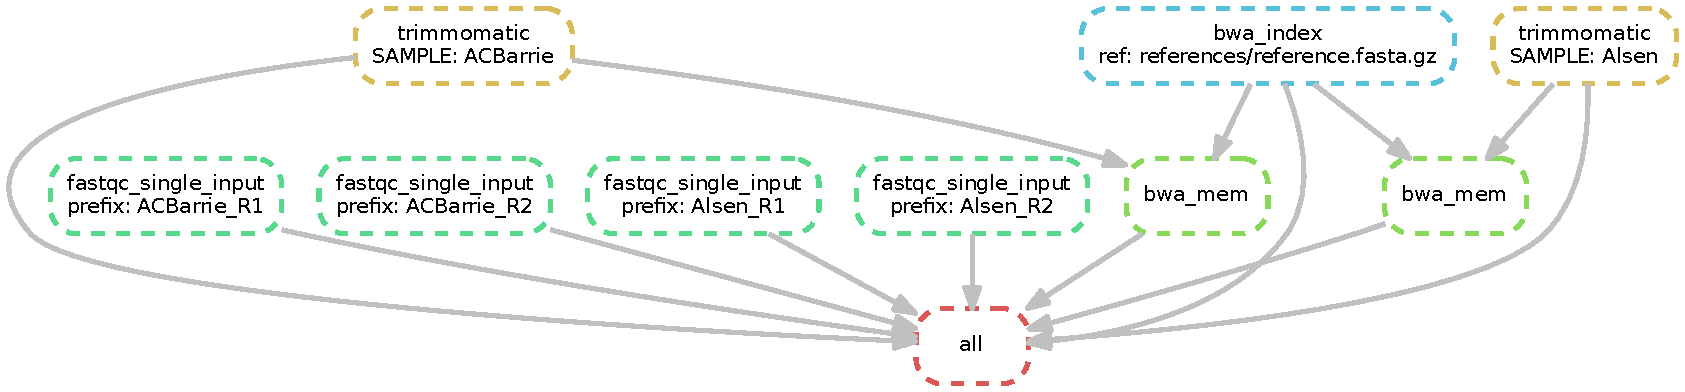
\includegraphics[width=0.8\textwidth]{handout/dag3.pdf}
\caption{DAG of jobs showing the dependencies which exist in our final implementation of the \texttt{analysis.sh} workflow.}
\label{fig:dag3}
\end{figure}

%------------------------
\subsection{Adding New Samples}
%------------------------

Our \texttt{SAMPLES} list contains a lot of samples which are currently commented out. Lets uncomment them and have a look
at some other features of Snakemake:

\begin{lstlisting}
# Manually uncomment the samples or use this sed command
sed -i 's/^# \{2\}"/  "/' Snakefile
\end{lstlisting}

With so many more samples, the DAG becomes next to useless with dot's default layout algorithm:

\begin{lstlisting}
# Generate a DAG
snakemake \
  --dag \
| dot -Tpdf \
> dag4.pdf
\end{lstlisting}

\begin{figure}[H]
\centering

\includegraphics[width=0.8\textwidth]{handout/dag4.pdf}
\caption{DAG of jobs for the whole workflow consisting of 16 samples.}
\label{fig:dag4}
\end{figure}

Instead, the ``rulegraph'' might provide a better view of the workflow. Unlike the DAG, that shows the individual jobs and their
dependencies, the rulegraph shows only the rules and and their dependencies so provides a simplified view of the workflow:

\begin{lstlisting}
# Generate a rulegraph
snakemake \
  --rulegraph \
| dot -Tpdf \
> rulegraph.pdf
\end{lstlisting}

\begin{figure}[H]
\centering
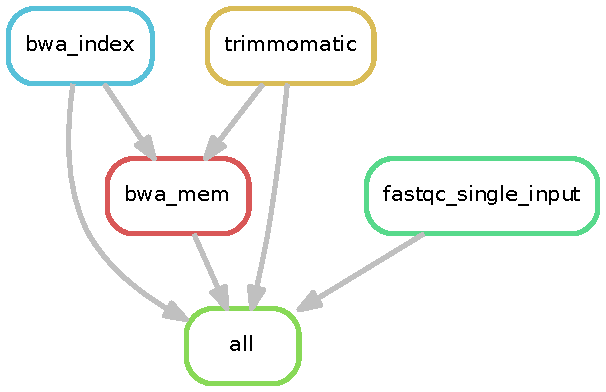
\includegraphics[width=0.8\textwidth]{handout/rulegraph.pdf}
\caption{Rulegraph for the whole workflow.}
\label{fig:rulegraph}
\end{figure}

Execute the rest of the workflow:

\begin{lstlisting}
# Execute the workflow
snakemake \
  --profile profiles/slurm \
  --use-singularity
\end{lstlisting}

In a different terminal, have a look at your jobs in the queue:

\begin{lstlisting}
sq
\end{lstlisting}

\begin{questions}

How many \texttt{fastqc} and total number of jobs are run as part of the whole workflow? Hint: try using \texttt{--forceall} in combination
with \texttt{--dryrun}.

\begin{answer}

\texttt{fastqc}: 32

Total: 66

\end{answer}

Using the Snakemake help, which command line argument can be used to get Snakemake to print the shell commands associated with each job during a \texttt{dryrun}?

\begin{answer}

\begin{lstlisting}
snakemake \
  --dryrun \
  --printshellcmds \
  --forceall
\end{lstlisting}

\end{answer}

Using the Snakemake help, which command line argument can be used to delete all the outputs associated with a given ``target''?

\begin{answer}

\begin{lstlisting}
snakemake \
  --delete-all-outputs
\end{lstlisting}

\end{answer}

\end{questions}

%------------------------
\subsection{Large Workflows}
%------------------------

A workflow I have developed is capable of mapping RNA-Seq, WGS, exome capture and Iso-Seq data to the wheat genome. In addition, downstream variant analysis and creation
of various tracks for JBrowse (e.g. BigWig) are possible. Much of the workflow involves broking the tasks down so each of the chromosomes is proccessed independantly, and
in parallel by the workflow. All up, there are more than 10,000 individual jobs representing 14 rules. DAG's of this size are best opened and layed out by Gephi using the
\texttt{ForceAtlas 2} algorithm:

\begin{figure}[H]
\centering
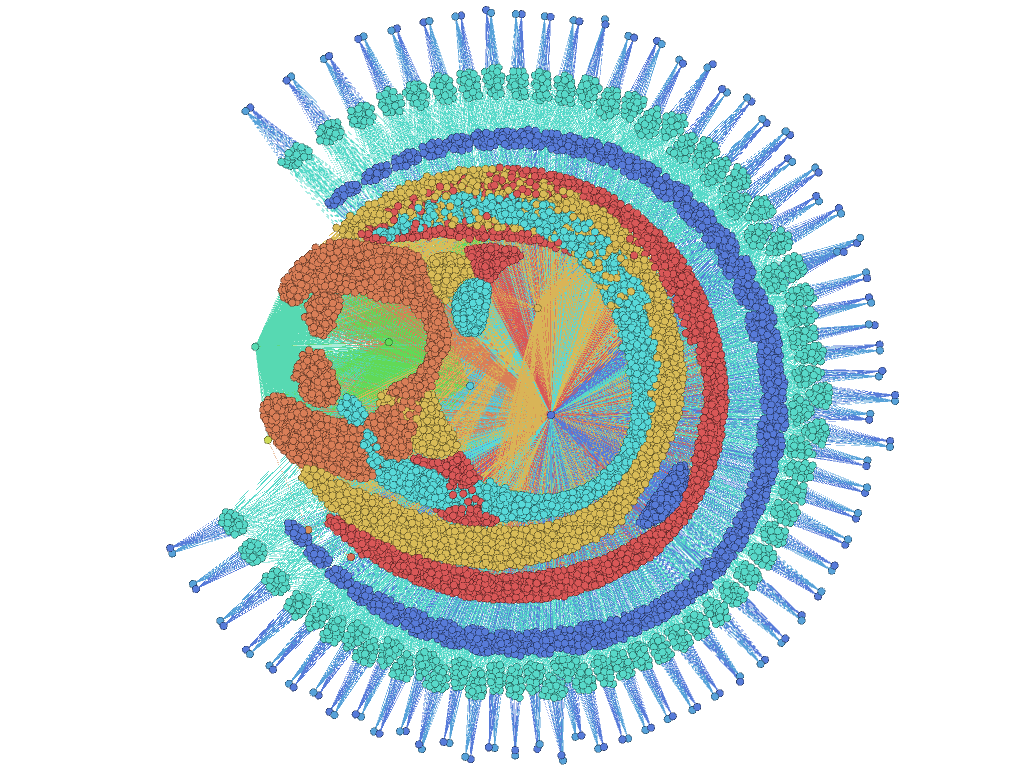
\includegraphics[width=0.8\textwidth]{handout/DAWN_DAG.png}
\caption{Large DAG, from the DAWN workflow, consisting of 10,587 nodes/jobs and 32,353 edges/dependancies. Layed out using \texttt{ForceAtlas 2} algorithm of Gephi}
\label{fig:dawn_dag}
\end{figure}

\begin{figure}[H]
\centering
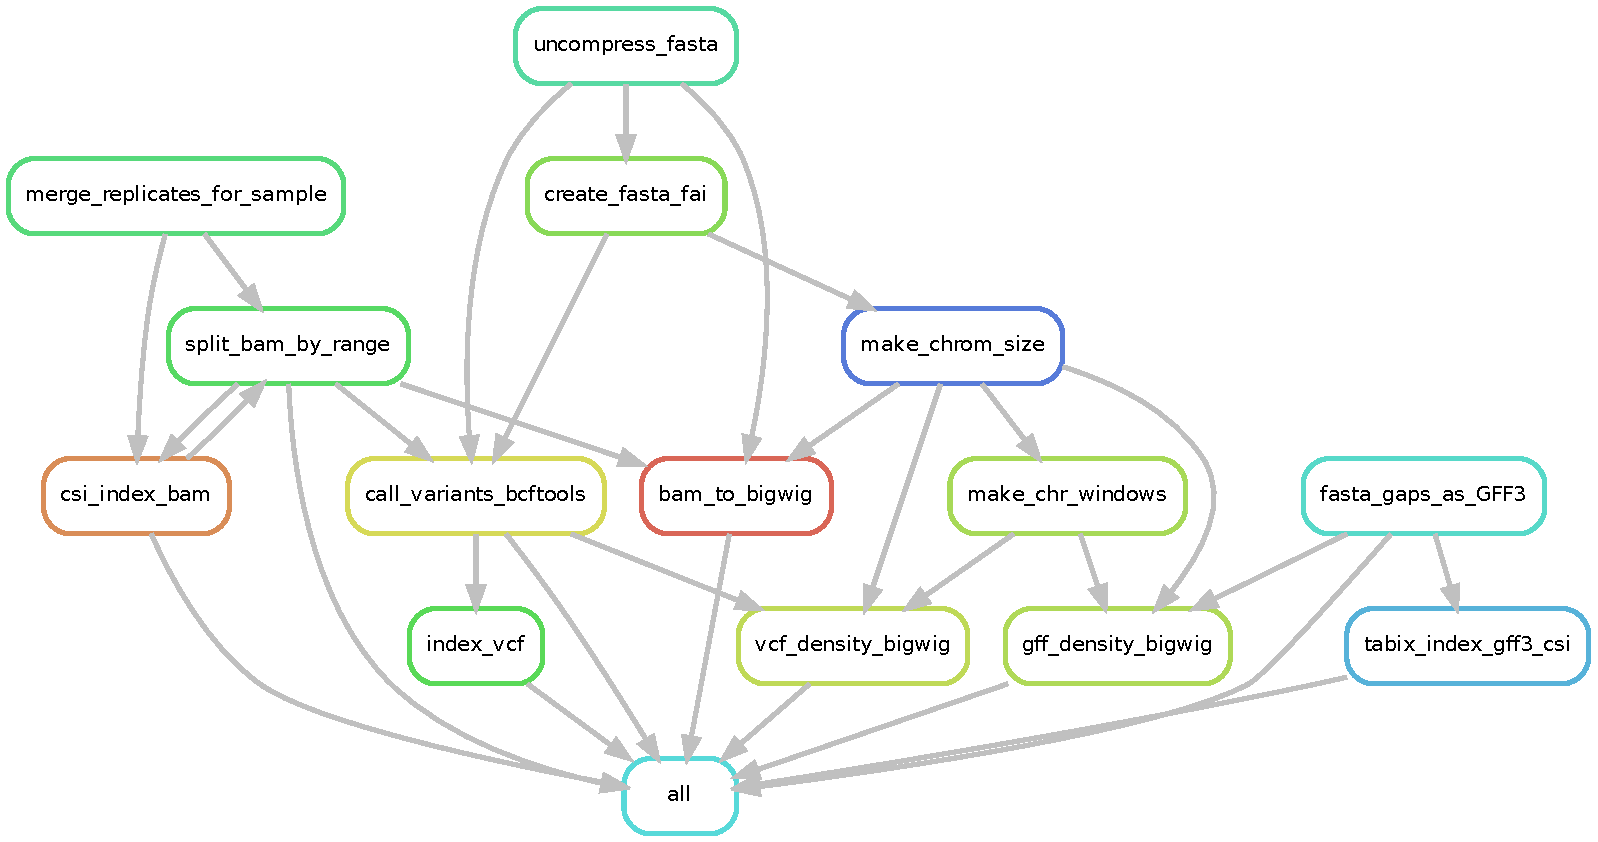
\includegraphics[width=0.8\textwidth]{handout/DAWN_rulegraph.pdf}
\caption{Rulegraph, from the DAWN workflow.}
\label{fig:dawn_rulegraph}
\end{figure}


%
% Possible Additions/Extensions:
%
%  Downloading files from remote sites: HTTP.remote
%


%========================
\newpage
\section{Snakemake Troubleshooting}
\label{sec:snake_trouble}
%========================

%------------------------
\subsection{Getting Going After a Disconnect}
%------------------------

If you find that your connection to the server has been dropped, you can get yourself going again using this convienient block of commands:

\begin{lstlisting}
# Load the required software modules
module load \
  miniconda3-4.6.14-gcc-5.4.0-kkzv7zk \
  singularity-3.2.1-gcc-5.4.0-tn5ndnb

# Activate the snakemake conda environment and
# integrate shell autocompletion into bash
conda activate snakemake
complete -o bashdefault -C snakemake-bash-completion snakemake

# Move to the correct directory location, most
# likely here:
cd /shared/${USER}/snakemake/tutorial
\end{lstlisting}
